%\documentclass[tikz]{standalone}
%\usetikzlibrary{positioning,chains}
%\usepackage{ifthen}
%\usepackage{tikz}
%\usetikzlibrary{arrows}
%\usetikzlibrary{decorations.markings}

%\begin{document}
\tikzset{
  big arrow/.style={
    decoration={markings,mark=at position 1 with {\arrow[scale=4,#1]{>}}},
    postaction={decorate},
    shorten >=0.4pt},
  big arrow/.default=blue}

\begin{tikzpicture}[node distance=0 cm,outer sep = 1pt,transform shape,scale=0.5]
    \tikzstyle{ML0} = [anchor=north east,circle, minimum width=1cm, minimum height=1cm, text centered, draw=black, fill=red!30]
    \tikzstyle{ML1} = [anchor=north east,circle, minimum width=1cm, minimum height=1cm, text centered, draw=black, fill=purple!30]
    \tikzstyle{ML2} = [anchor=north east,circle, minimum width=1cm, minimum height=1cm, text centered, draw=black, fill=green!30]
    \tikzstyle{ML} = [anchor=north east,rectangle, minimum width=21em, minimum height=1cm, text width=2cm, text centered, draw=black, fill=orange!30]
    \node (i1) at (2.7,1.2)  [rectangle, align=center, draw, very thick, fill=red!10, minimum height=12em, minimum width=21em] {};
    \foreach \x in {0,...,4}
      \foreach \y in {0,...,2}
      {\pgfmathtruncatemacro{\label}{Mod(\x - 5 *  \y +21,3 )}
	\ifthenelse{\label = 0}
    {\node [ML0]  (\x\y) at (1.5*\x,1.5*\y) {T1}}
    {\ifthenelse{\label = 1} 
{\node [ML1]  (\x\y) at (1.5*\x,1.5*\y) {T2}}
{\node [ML2]  (\x\y) at (1.5*\x,1.5*\y) {Free}}
}
    ;}
    \node (c2)  [ML,above=of i1] {Softmax(X/10)};
    \node (c3) at (2.7,6.2) {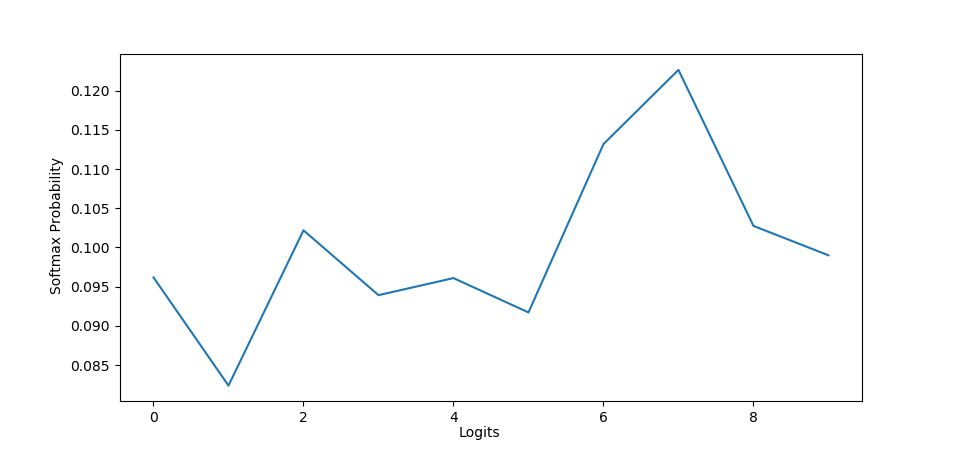
\includegraphics[width=16em]{temp_10.png}};
    \draw[red, big arrow]  (2.5,5) -- (2.5,3);
    \draw[red, big arrow]  (1,5) -- (1,3);
    \draw[red, big arrow]  (4,5) -- (4,3);

\end{tikzpicture}

%\end{document}
